% Hlavicka pro protokoly z fyzikalniho praktika.
% Verze pro: LaTeX
% Verze hlavicky: 22. 2. 2007
% Autor: Ustav fyziky kondenzovanych latek
% Ke stazeni: www.physics.muni.cz/ufkl/Vyuka/
% Licence: volne k pouziti, nejlepe k vcasnemu odevzdani protokolu z Vaseho mereni.


\documentclass[czech,11pt,a4paper]{article}
\usepackage[T1]{fontenc}
\usepackage{graphicx, animate}
\usepackage{mathtools}
\usepackage{amssymb}
\usepackage{amsthm}
\usepackage{thmtools}
\usepackage{diagbox, xcolor}
\usepackage{xcolor}
\usepackage{nameref}
\usepackage{babel}
\usepackage{hyperref}
\usepackage{multicol}
\usepackage[export]{adjustbox}
\usepackage{subcaption}
\usepackage{caption}
\usepackage{multirow}
\usepackage{float}
\usepackage{placeins}
\graphicspath{ {./images/} }



%%% Nemente:
\usepackage[margin=2cm]{geometry}
\newtoks\jmenopraktika \newtoks\jmeno \newtoks\datum
\newtoks\obor \newtoks\skupina \newtoks\rocnik \newtoks\semestr
\newtoks\cisloulohy \newtoks\jmenoulohy
\newtoks\tlak \newtoks\teplota \newtoks\vlhkost
%%% Nemente - konec.


%%%%%%%%%%% Doplnte pozadovane polozky:

\jmenopraktika={Fyzikální praktikum 2}  % nahradte jmenem vaseho predmetu
\jmeno={Teodor Duraković}            % nahradte jmenem mericiho
\datum={14.~října 2024}        % nahradte datem mereni ulohy
\obor={F}                     % nahradte zkratkou vami studovaneho oboru
\skupina={Po 14:00}            % nahradte dobou vyuky vasi seminarni skupiny
\rocnik={II}                  % nahradte rocnikem, ve kterem studujete
\semestr={III}                 % nahradte semestrem, ve kterem studujete

\cisloulohy={3}               % nahradte cislem merene ulohy
\jmenoulohy={Rozložení elektrického pole} % nahradte jmenem merene ulohy

\tlak={ 968}                   % nahradte tlakem pri mereni (v hPa)
\teplota={23.3}               % nahradte teplotou pri mereni (ve stupnich Celsia)
\vlhkost={41}               % nahradte vlhkosti vzduchu pri mereni (v %)

%%%%%%%%%%% Konec pozadovanych polozek.


%%%%%%%%%%% Uzitecne balicky:

%%%%%% Zamezeni parchantu:
\widowpenalty 10000 \clubpenalty 10000 \displaywidowpenalty 10000
%%%%%% Parametry pro moznost vsazeni vetsiho poctu obrazku na stranku
\setcounter{topnumber}{3}	  % max. pocet floatu nahore (specifikace t)
\setcounter{bottomnumber}{3}	  % max. pocet floatu dole (specifikace b)
\setcounter{totalnumber}{6}	  % max. pocet floatu na strance celkem
\renewcommand\topfraction{0.9}	  % max podil stranky pro floaty nahore
\renewcommand\bottomfraction{0.9} % max podil stranky pro floaty dole
\renewcommand\textfraction{0.1}	  % min podil stranky, ktery musi obsahovat text
\intextsep=8mm \textfloatsep=8mm  %\intextsep pro ulozeni [h] floatu a \textfloatsep pro [b] or [t]

% Tecky za cisly sekci:
\renewcommand{\thesection}{\arabic{section}.}
\renewcommand{\thesubsection}{\thesection\arabic{subsection}.}
\renewcommand{\thesubsubsection}{\thesubsection\arabic{subsubsection}.}
% Jednopismenna mezera mezi cislem a nazvem kapitoly:
\makeatletter \def\@seccntformat#1{\csname the#1\endcsname\hspace{1ex}} \makeatother


%%%%%%%%%%%%%%%%%%%%%%%%%%%%%%%%%%%%%%%%%%%%%%%%%%%%%%%%%%%%%%%%%%%%%%%%%%%%%%%
%%%%%%%%%%%%%%%%%%%%%%%%%%%%%%%%%%%%%%%%%%%%%%%%%%%%%%%%%%%%%%%%%%%%%%%%%%%%%%%
% Zacatek dokumentu
%%%%%%%%%%%%%%%%%%%%%%%%%%%%%%%%%%%%%%%%%%%%%%%%%%%%%%%%%%%%%%%%%%%%%%%%%%%%%%%
%%%%%%%%%%%%%%%%%%%%%%%%%%%%%%%%%%%%%%%%%%%%%%%%%%%%%%%%%%%%%%%%%%%%%%%%%%%%%%%

\begin{document}
	
	%%%%%%%%%%%%%%%%%%%%%%%%%%%%%%%%%%%%%%%%%%%%%%%%%%%%%%%%%%%%%%%%%%%%%%%%%%%%%%%
	% Nemente:
	%%%%%%%%%%%%%%%%%%%%%%%%%%%%%%%%%%%%%%%%%%%%%%%%%%%%%%%%%%%%%%%%%%%%%%%%%%%%%%%
	\thispagestyle{empty}
	
	{
		\begin{center}
			\sf 
			{\Large Ústav fyzikální elektroniky Přírodovědecké fakulty Masarykovy univerzity} \\
			\bigskip
			{\huge \bfseries FYZIKÁLNÍ PRAKTIKUM} \\
			\bigskip
			{\Large \the\jmenopraktika}
		\end{center}
		
		\bigskip
		
		\sf
		\noindent
		\setlength{\arrayrulewidth}{1pt}
		\begin{tabular*}{\textwidth}{@{\extracolsep{\fill}} l l}
			\large {\bfseries Zpracoval:}  \the\jmeno & \large  {\bfseries Naměřeno:} \the\datum\\[2mm]
			\large  {\bfseries Obor:} \the\obor  \hspace{40mm}  {\bfseries Skupina:} \the\skupina %
			%{\bfseries Ročník:} \the\rocnik \hspace{5mm} {\bfseries Semestr:} \the\semestr  
			&\large {\bfseries Testováno:}\\
			\\
			\hline
		\end{tabular*}
	}
	
	\bigskip
	
	{
		\sf
		\noindent \begin{tabular}{p{3cm} p{0.6\textwidth}}
			\Large  Úloha č. {\bfseries \the\cisloulohy:} \par
			\smallskip
			$T=\the\teplota$~$^\circ$C \par
			$p=\the\tlak$~hPa \par
			$\varphi=\the\vlhkost$~\%
			&\Large \bfseries \the\jmenoulohy  \\[2mm]
		\end{tabular}
	}
	
	\vskip1cm
	
	%%%%%%%%%%%%%%%%%%%%%%%%%%%%%%%%%%%%%%%%%%%%%%%%%%%%%%%%%%%%%%%%%%%%%%%%%%%%%%%
	% konec Nemente.
	%%%%%%%%%%%%%%%%%%%%%%%%%%%%%%%%%%%%%%%%%%%%%%%%%%%%%%%%%%%%%%%%%%%%%%%%%%%%%%%
	
	%%%%%%%%%%%%%%%%%%%%%%%%%%%%%%%%%%%%%%%%%%%%%%%%%%%%%%%%%%%%%%%%%%%%%%%%%%%%%%%
	%%%%%%%%%%%%%%%%%%%%%%%%%%%%%%%%%%%%%%%%%%%%%%%%%%%%%%%%%%%%%%%%%%%%%%%%%%%%%%%
	% Zacatek textu vlastniho protokolu
	%%%%%%%%%%%%%%%%%%%%%%%%%%%%%%%%%%%%%%%%%%%%%%%%%%%%%%%%%%%%%%%%%%%%%%%%%%%%%%%
	%%%%%%%%%%%%%%%%%%%%%%%%%%%%%%%%%%%%%%%%%%%%%%%%%%%%%%%%%%%%%%%%%%%%%%%%%%%%%%%
	\begin{multicols}{2}
		

	\section{Zadání}
	1. Pochopení a praktické zvládnutí měření rozložení elektrického pole v elektrolytické vaně pomocí střídavého mostu.\\
	2. Osvojení si schopnosti sestavení měřícího obvodu a přizpůsobení nastavení osciloskopu cílům měření.\\
	3. Porovnání měřeného elektrostatického pole v okolí dvouvodičového vedení s teoretickým výpočtem.\\
	
	
	\section{Teorie}
	\section*{Rozložení potenciálu v okolí dvouvodičového vedení}
	\section*{Teoretický úvod}
	Potenciál pole ve vzdálenosti $r$ od přímého vodiče s lineární hustotou náboje $\tau$ je
	
	
	\begin{equation*}
		V=\frac{\tau}{2 \pi \epsilon} \ln \frac{R}{r} \tag{3.1}
	\end{equation*}
	
	
	kde $R$ je vzdálenost od vodiče, ve které klademe potenciál roven nule $V(R)=0$ (nelze volit $V(\infty)=0$, protože náboj je rozložen na vodiči, jehož délka není omezena). Volíme-li místo nulového potenciálu ve vzdálenosti $R=1 \mathrm{~m}$ od vodiče, pak můžeme vztah (3.1) psát
	
	
	\begin{equation*}
		V=-\frac{\tau}{2 \pi \epsilon} \ln r \tag{3.2}
	\end{equation*}
	
	
	\begin{figure}[H]
		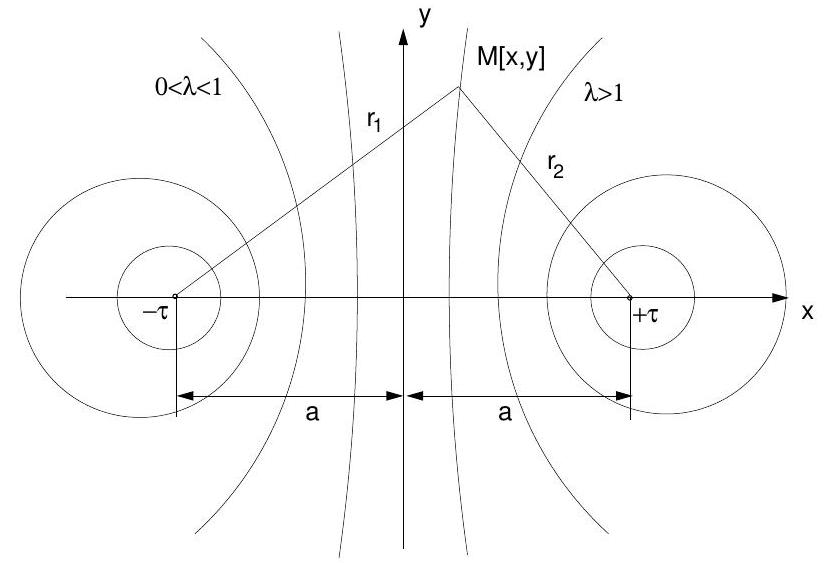
\includegraphics[max width=0.5\textwidth]{2024_10_15_71c3161fc9161f95056eg-1}
		\caption{Ekvipotenciální hladiny v rovině kolmé na dva rovnoběžné nekonečně dlouhé nabité vodiče.}
	\end{figure}
	
	
	Potenciál v bodě $M$ (3.1) od dvou lineárních rovnoběžných vodičů je podle principu superpozice s přihlédnutím ke vztahu (3.2) dán
	
	
	\begin{equation*}
		V=V_{1}+V_{2}=\frac{\tau}{2 \pi \epsilon} \ln \frac{r_{2}}{r_{1}} \tag{3.3}
	\end{equation*}
	
	
	Na vodičích jsou rozloženy elektrické náboje s konstantními lineárními hustotami $+\tau$ a $-\tau$. Pro ekvipotenciály platí
	
	
	\begin{equation*}
		\frac{\tau}{2 \pi \epsilon} \ln \frac{r_{2}}{r_{1}}=\text { konst., } \quad \text { nebo } \quad \frac{r_{2}}{r_{1}}=\lambda \tag{3.4}
	\end{equation*}
	
	
	kde $r_{1}=\sqrt{(a-x)^{2}+y^{2}}, r_{2}=\sqrt{(a+x)^{2}+y^{2}}$ a $\lambda>0$ je parametr ekvipotenciálních hladin.\\
	Geometrickým místem bodů v rovině, které mají od daných dvou bodů konstantní poměr vzdáleností $\lambda$, je pro $\lambda=1$ přímka a pro $\lambda \neq 1$ Apolloniova kružnice. Ve zvolené soustavě kartézských souřadnic je touto přímkou osa $y$, středy $S\left[x_{s}, 0\right]$ a poloměry $r$ Apolloniových kružnic určíme tak, že rovnice (3.4) upravíme na tvar
	
	
	\begin{equation*}
		\left(x-a \frac{\lambda^{2}+1}{\lambda^{2}-1}\right)^{2}+y^{2}=a^{2}\left(\frac{\lambda^{2}+1}{\lambda^{2}-1}\right)^{2}-a^{2} \tag{3.5}
	\end{equation*}
	
	
	Pak
	
	
	\begin{equation*}
		x_{s}=a \frac{\lambda^{2}+1}{\lambda^{2}-1}, \quad r=\sqrt{x_{s}^{2}-a^{2}} \tag{3.6}
	\end{equation*}
	
	
	Z prvních tří rovnic (3.21) plyne pro potenciál elektrostatického pole Laplaceova rovnice
	
	
	\begin{equation*}
		\nabla^{2} V=0 \tag{3.7}
	\end{equation*}
	
	
	Problém určení elektrostatického pole dvojvodičového vedení tvořeného rovnoběžnými válcovými vodiči nahradíme řešením elektrostatického pole dvojice rovnoběžných vodičů. Okrajové podmínky zachováme, postupujeme-li takto: dané válcové vodiče nahradíme válci z dielektrika s permitivitou prostředí $\epsilon$ a do každého z nich vložíme přímkový vodič s lineární hustotou náboje $\tau$, resp. $-\tau$ (obrázek 2), tzv. elektrické osy.\\
	\begin{figure}[H]
		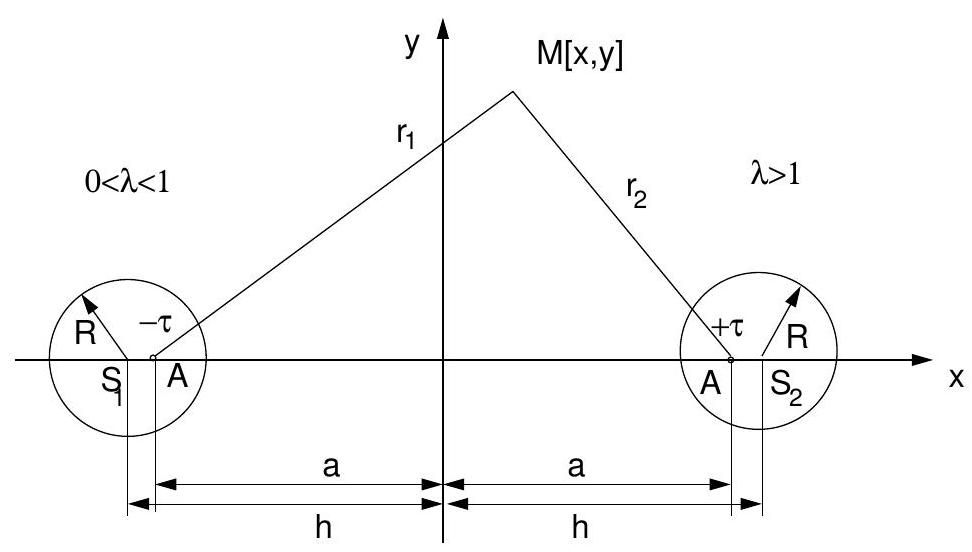
\includegraphics[max width=0.5\textwidth, center]{2024_10_15_71c3161fc9161f95056eg-2}
		
		\caption{ Výpočet potenciálu v bodě $M$ od dvou válcových nekonečných vodičů s poloměrem $R$, mezi nimiž je rozdíl potenciálů $U$.}
	\end{figure}
	
	
	Polohu os a hodnotu $\tau$ stanovíme tak, aby elektrické pole, které vytvářejí, mělo ekvipotenciální plochy $V_{1}$ a $V_{2}$ s poloměry $R$ právě v místech povrchu válců, přičemž musí být $V_{1}-V_{2}=U$. Ve zvolené souřadné soustavě je vzdálenost středů $S_{1}$ a $S_{2}$ vodivých válců $2 h$, pak poloha náhradních vodičů $A$ a $B$ se určí z rovnice 3.6
	
	
	\begin{equation*}
		a=\sqrt{h^{2}-R^{2}} \tag{3.8}
	\end{equation*}
	
	
	Z poslední rovnice je zřejmé, že body $A$ a $B$ jsou vzájemně sdružené v kulové inverzi vzhledem ke kružnicím se středy $S_{1}$ a $S_{2}$. Pak platí
	
	{\small 
	\begin{equation*} 
		R^{2}=h^{2}-a^{2}=(h-a)(h+a)=\overline{S_{2} A} \cdot \overline{S_{2} B}=\overline{S_{1} B} \cdot \overline{S_{1} A} \tag{3.9}
	\end{equation*}}
	
	
	Potenciál v bodě $M$ bude podle 3.3
	
	
	\begin{equation*}
		V=\frac{\tau}{2 \pi \epsilon} \ln \frac{r_{2}}{r_{1}}=\frac{\tau}{2 \pi \epsilon} \ln \lambda \tag{3.10}
	\end{equation*}
	
	
	Pro potenciály na ekvipotenciálních plochách totožných s válcovými vodiči dostaneme podle 3.10 s použitím 3.9 .
	
	
	\begin{gather*}
		V_{1} \equiv \frac{\tau}{2 \pi \epsilon} \ln \frac{\overline{A P}}{\overline{B P}}=\frac{\tau}{2 \pi \epsilon} \ln \frac{h+a}{R}, \quad \\ V_{2} \equiv \frac{\tau}{2 \pi \epsilon} \ln \frac{\overline{A Q}}{\overline{B Q}}=\frac{\tau}{2 \pi \epsilon} \ln \frac{R}{h+a} \tag{3.11}
	\end{gather*}
	
	
	Hodnotu $\tau$ určíme z podmínky $U=V_{1}-V_{2}$
	
	
	\begin{equation*}
		\tau=\frac{\pi \epsilon U}{\ln \frac{h+a}{R}} \tag{3.12}
	\end{equation*}
	
	
	Dosazením 3.12 do 3.10 dostaneme
	
	
	\begin{equation*}
		V=\frac{U}{2 \ln \frac{h+a}{R}} \ln \frac{r_{2}}{r_{1}} \tag{3.13}
	\end{equation*}
	
	
	Rovnice 3.10 je odvozena pro symetrické rozložení nábojů, které v běžném experimentálním uspořádání není splněno (obyčejně máme $V_{1}=U$ a $V_{2}=0$ nebo naopak a nikoliv $V_{1}=U / 2$ a $\left.V_{2}=-U / 2\right)$. Ve shodě s naším experimentálním uspořádáním posuneme hladinu, od které počítáme potenciál, o $U / 2$, tedy
	
	
	\begin{equation*}
		V=\frac{U}{2 \ln \frac{h+a}{R}} \ln \frac{r_{2}}{r_{1}}+\frac{U}{2} \tag{3.14}
	\end{equation*}
	
	
	Parametr $\lambda$ příslušející konkrétní ekvipotenciální hladině s potenciálem $V$ pak vypočteme jako
	
	
	\begin{equation*}
		\ln \lambda=\frac{V-\frac{U}{2}}{U} 2 \ln \frac{h+a}{R}=\left(\frac{V}{U}-\frac{1}{2}\right) 2 \ln \frac{h+a}{R} \tag{3.15}
	\end{equation*}
	
	
	\section*{Měření rozložení elektrostatického pole}
	Elektrostatické pole je svou podstatou vektorovým polem, tvořeným vektorem intenzity $\boldsymbol{E}$. Můžeme je však stejně dobře popsat, užijeme-li skalárního pole hodnot elektrostatického potenciálu $V$. Uvedené vektorové pole intenzity a skalární pole potenciálu jsou si zcela ekvivalentní a platí
	
	
	\begin{equation*}
		\boldsymbol{E}=-\nabla V \tag{3.16}
	\end{equation*}
	
	
	Ekvipotenciální hladinou se nazývá v obecném případě plocha, na které má potenciál všude stejnou hodnotu
	
	
	\begin{equation*}
		V(x, y, z)=V_{0}=\text { konst } \tag{3.17}
	\end{equation*}
	
	
	Pro každý elementární posuv $\delta x, \delta y, \delta z$ po této ploše platí zřejmě podmínky $\delta V=0$ a tedy také
	
	
	\begin{equation*}
		-\left(E_{x} \delta x+E_{y} \delta y+E_{z} \delta z\right)=-\boldsymbol{E} \cdot \delta \boldsymbol{l}=0 \tag{3.18}
	\end{equation*}
	
	
	Tato rovnice říká, že skalární součin intenzity s libovolným posunem po hladině je nulový, tj. intenzita je všude kolmá k ekvipotenciálním hladinám a siločáry jimi probíhají kolmo.
	
	Vztah (3.16) vede ryze matematickým postupem k další důležité rovnici
	
	
	\begin{equation*}
		\operatorname{rot} \boldsymbol{E}=0 \tag{3.19}
	\end{equation*}
	
	
	tedy elektrostatické pole je pole nevírové. V místech bez náboje je také
	
	
	\begin{equation*}
		\operatorname{div} \boldsymbol{E}=0 \tag{3.20}
	\end{equation*}
	
	
	to znamená, že uvažované pole je nezřídlové.\\
	Měření rozložení potenciálu v elektrostatickém poli je z experimentálního hlediska dosti obtížné. Využívá se proto analogie mezi elektrostatickým polem v homogenním dielektriku a elektrickým polem uvnitř homogenního vodiče, kterým protéká stacionární proud. V jednotlivých případech je pole popsáno:
	
	Pole stacionárního proudu Elektrostatické pole
	
	\[
	\begin{array}{rc}
		\boldsymbol{E}_{s}=-\nabla V_{s} & \boldsymbol{E}_{e}=-\nabla V_{e}  \tag{3.21}\\
		\boldsymbol{j}_{s}=\sigma \boldsymbol{E}_{s} & \boldsymbol{D}_{e}=\epsilon \boldsymbol{E}_{e} \\
		\operatorname{div} \boldsymbol{j}_{s}=0 & \operatorname{div} \boldsymbol{D}_{e}=0 \\
		\oint \boldsymbol{E}_{s} \cdot \mathrm{~d} \boldsymbol{l}=0 & \oint \boldsymbol{E}_{e} \cdot \mathrm{~d} \boldsymbol{l}=0
	\end{array}
	\]
	
	kde $\boldsymbol{E}_{s}, \boldsymbol{E}_{e}$ je vektor intenzity pole, $\boldsymbol{j}_{s}$ proudová hustota, $\boldsymbol{D}_{e}$ vektor elektrostatické indukce, $\sigma$ vodivost prostředí, ve kterém teče proud, $\epsilon$ permitivita prostředí, v němž se elektrostatické pole vyskytuje. Za předpokladu, že dielektrikum je homogenní a neexistují v něm volné náboje a vodič je homogenní $(\sigma=$ konst. $\neq 0$ ), jsou soustavy rovnic 3.21 pro pole stacionárního proudu a elektrostatické pole zcela ekvivalentní. Pak lze elektrostatické pole trojrozměrného systému v prostředí s permitivitou $\epsilon$ studovat jako pole proudu $\boldsymbol{j}_{s} \mathrm{v}$ prostředí s vodivostí $\sigma$. Měření obyčejně provádíme v rovině, tj. studujeme takové trojrozměrné systémy, které mohou být popsány rozložením pole v určité rovině. Jsou to jednak systémy nezávislé na jedné ze souřadných os a jednak systémy, které mají rotační symetrii. Poslední případ se týká např. elektrostatických čoček.
	
	
	\section*{Postup měření:}
	Měření se provádí v elektrolytické vaně zapojené jako střídavý můstek. Je to nevodivá nádoba se slabým elektrolytem, do níž se umístí modely vodičù, jejichž elektrické pole chceme vyšetřovat. Rozměry nádoby je nutno volit tak, aby hustota proudu u jejich stěn byla mnohem menší než v prostoru, kde měříme. Na obrázku 3 je schéma zapojení vany do střídavého mostu se dvěma elektrodami $M_{1}$ a $M_{2}$. Oba kanály osciloskopu jsou připojeny k obvodu pomocí koaxiálních kabelů, jejichž stínící vodiče propojují zemněný vodič generátoru se zemí osciloskopu. Sondou (S) je kovová jehla sloužící k mapování potenciálu ve vaně. Sonda je připevněna k pantografu přes nějž je poloha jehly přenášena do grafického tabletu a z něj do měřícího programu běžícího na PC. Dále je sonda spojena s kanálem 1 osciloskopu. Kanál 2 osciloskopu je připojen k jezdci potenciometru, pomocí něhož nastavujeme referenční potenciál. Osciloskop je pak nastaven v režimu měření rozdílu signálů na kanálech $1 \,\mathrm{ a}\, 2, \mathrm{tj} .{ }{1}-2$. Nastavený potenciálový rozdíl mezi zemí obvodu a jezdcem potenciometru je měřen pomocí voltmetru.
	
	Sondou $S$ hledáme ta místa v elektrolytu, jejichž potenciál je stejný jako potenciál $U_{1}$ nastavený na potenciometru $\left(S_{1}\right)$. Je-li potenciál sondy a jezdce potenciometru stejný, pak osciloskop vykazuje minimální signál. To odpovídá přibližně rovné čáře na osciloskopu.
	
	Pomocí odečítacího zařízení (pantografu) lze postupně přes grafický tablet přenést do ovládacího programu na PC sít bodů o stejném potenciálu. Jejich spojením dostáváme průběh ekvipotenciální čáry. Siločáry jsou v každém bodě kolmé k ekvipotenciálním čarám: takovým způsobem lze postupně zmapovat průběh elektrostatického pole v určité rovině.\\
	\begin{figure}[H]
		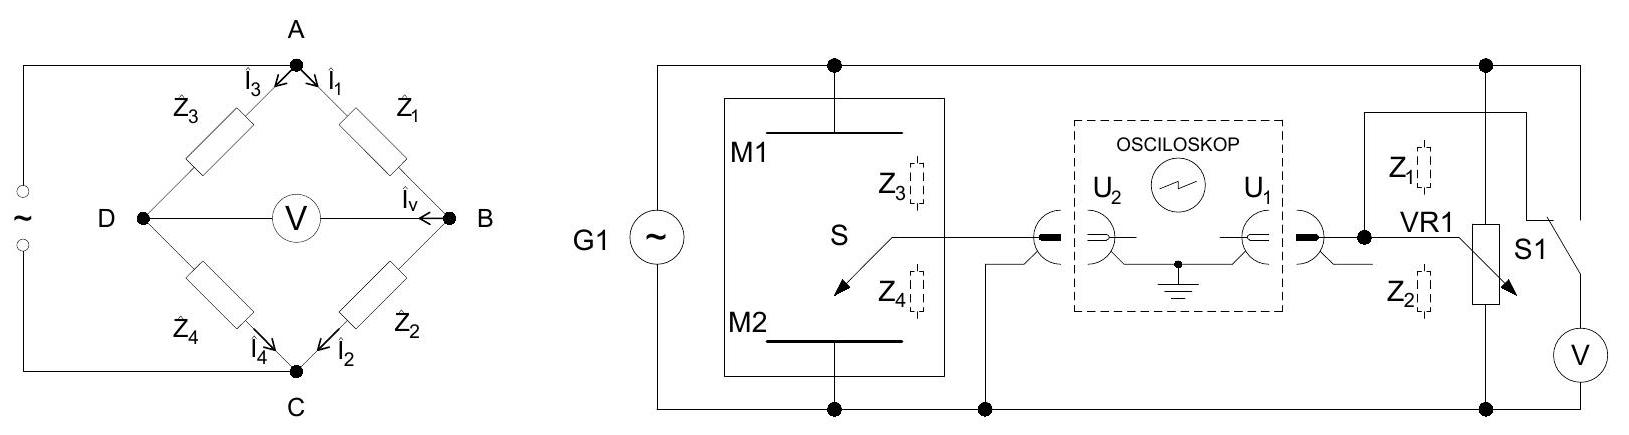
\includegraphics[max width=0.5\textwidth, center]{2024_10_15_71c3161fc9161f95056eg-5}
		\caption{Obecný střídavý můstek (vlevo). Zapojení střídavého můstku pro měření v elektrolytické vaně (vpravo) se zakreslenými ekvivalenty impedancí v levém obrázku (čerchovaně zakreslené značky rezistoru). Osciloskop je k obvodu připojen přes koaxiální kabely, jejichž stínící vodiče propojují zemněný vodič generátoru se zemí osciloskopu.}
	\end{figure}
	
	Měření zpravidla provádíme střídavým proudem. Vyhneme se tím možné chybě způsobené polarizací elektrod . Je-li frekvence střídavého proudu $10^{2}$ až $10^{3} \mathrm{~Hz}$, pracujeme v podstatě s kvazistacionárními proudy a ekvivalentnost systému rovnic 3.21 je splněna v tomto případě
	

	s dostatečnou přesností. Popsaná metoda je již poněkud překonaná moderními metodami, poskytuje však velmi dobrou představu o průběhu ekvipotenciálních čar v sestavené konfiguraci. Je-li napětí na elektrodách $\sim 10 \mathrm{~V}$ a detektorem lze měřit změny napětí řádově $10^{-2} \mathrm{~V}$, určíme polohu ekvipotenciálních čar s přesností asi $1 \%$ .
	
	
	
	\section{Měření}
	Po změření dimenzí elektrod a jejich vzájemné vzdálenosti získáme hodnoty:
	\begin{gather*}
		R = 1.5\,\mathrm{cm} \\
		h = 14.9\,\mathrm{cm} \\
		a = \sqrt{h^2 - R^2} = 14.8\,\mathrm{cm},		
	\end{gather*}
	kde $R$ je poloměr elektrody, $h$ vzdálenost jejich středů a $a$ je vzdálenost polohy náhradních vodičů od počátku souřadnic. Budeme měřit 9 ekvipotenciálních hladin, a to od napětí $U_1 = 0.5 \,\rm V$ po napětí $U_9 = 4.5\,\rm V$ s inkrementem $0.5\,\rm V$. Pomocí formule (3.15) získáme jednotlivé hodnoty $\lambda$ pro jmenovité hodnoty napětí. 
	Formuli (3.6) použijeme pro kalkulaci poloměrů a poloh středů Apolloniových kružnic. Získáváme hodnoty:
	
	\begin{tabular}{|c|c|c|c|}\hline
		$U$ [V] & $\lambda$ & $x_s$[cm] & $\mathrm{r}[\mathrm{cm}]$ \\\hline
		0.5 & 0.091802 & -15.055852 & 2.741216 \\ \hline
		1.0 & 0.166778 & -15.651323 & 5.079320 \\\hline
		1.5 & 0.302989 & -17.797068 & 9.877815 \\\hline
		2.0 & 0.550444 & -27.674882 & 23.382359 \\\hline
		2.5 & 1.000000 & $\infty$ & $\infty$ \\\hline
		3.0 & 1.816715 & 27.674882 & 23.382359 \\\hline
		3.5 & 3.300454 & 17.797068 & 9.877815 \\\hline
		4.0 & 5.995984 & 15.651323 & 5.079320 \\\hline
		4.5 & 10.892995 & 15.055852 & 2.741216 \\ \hline
	\end{tabular}
	\\
	Zde je nutno porozumět výsledkům pro napěťovou hladinu $2.5$ V. Křivku s nekonečným poloměrem křivosti můžeme chápat jako přímku, která se musí v souladu s teorií nacházet uprostřed mezi vodiči, tvoříc osu, dle které jsou ostatní kružnice souměrné. Toto si můžeme ověřit studií okolí hladiny $2.5$V:	
\begin{figure}[H]
		\begin{center}
			\animategraphics[autoplay, loop, width=1\linewidth]{30}{plot_}{0}{49}
			\caption{Apolloniovy kružnice pro hladiny blízké $2.5$ V (\textit{K správnému zobrazení animace je nutno dokument otevřít v programu, který animace podporuje (kupř. Adobe Acrobat)})}
	
		\end{center}
\end{figure}
\newpage
Po ověření našeho předpokladu můžeme vynést do grafu naměřené hodnoty spolu se získanými kružnicemi:
\begin{figure}[H]
	\begin{center}
		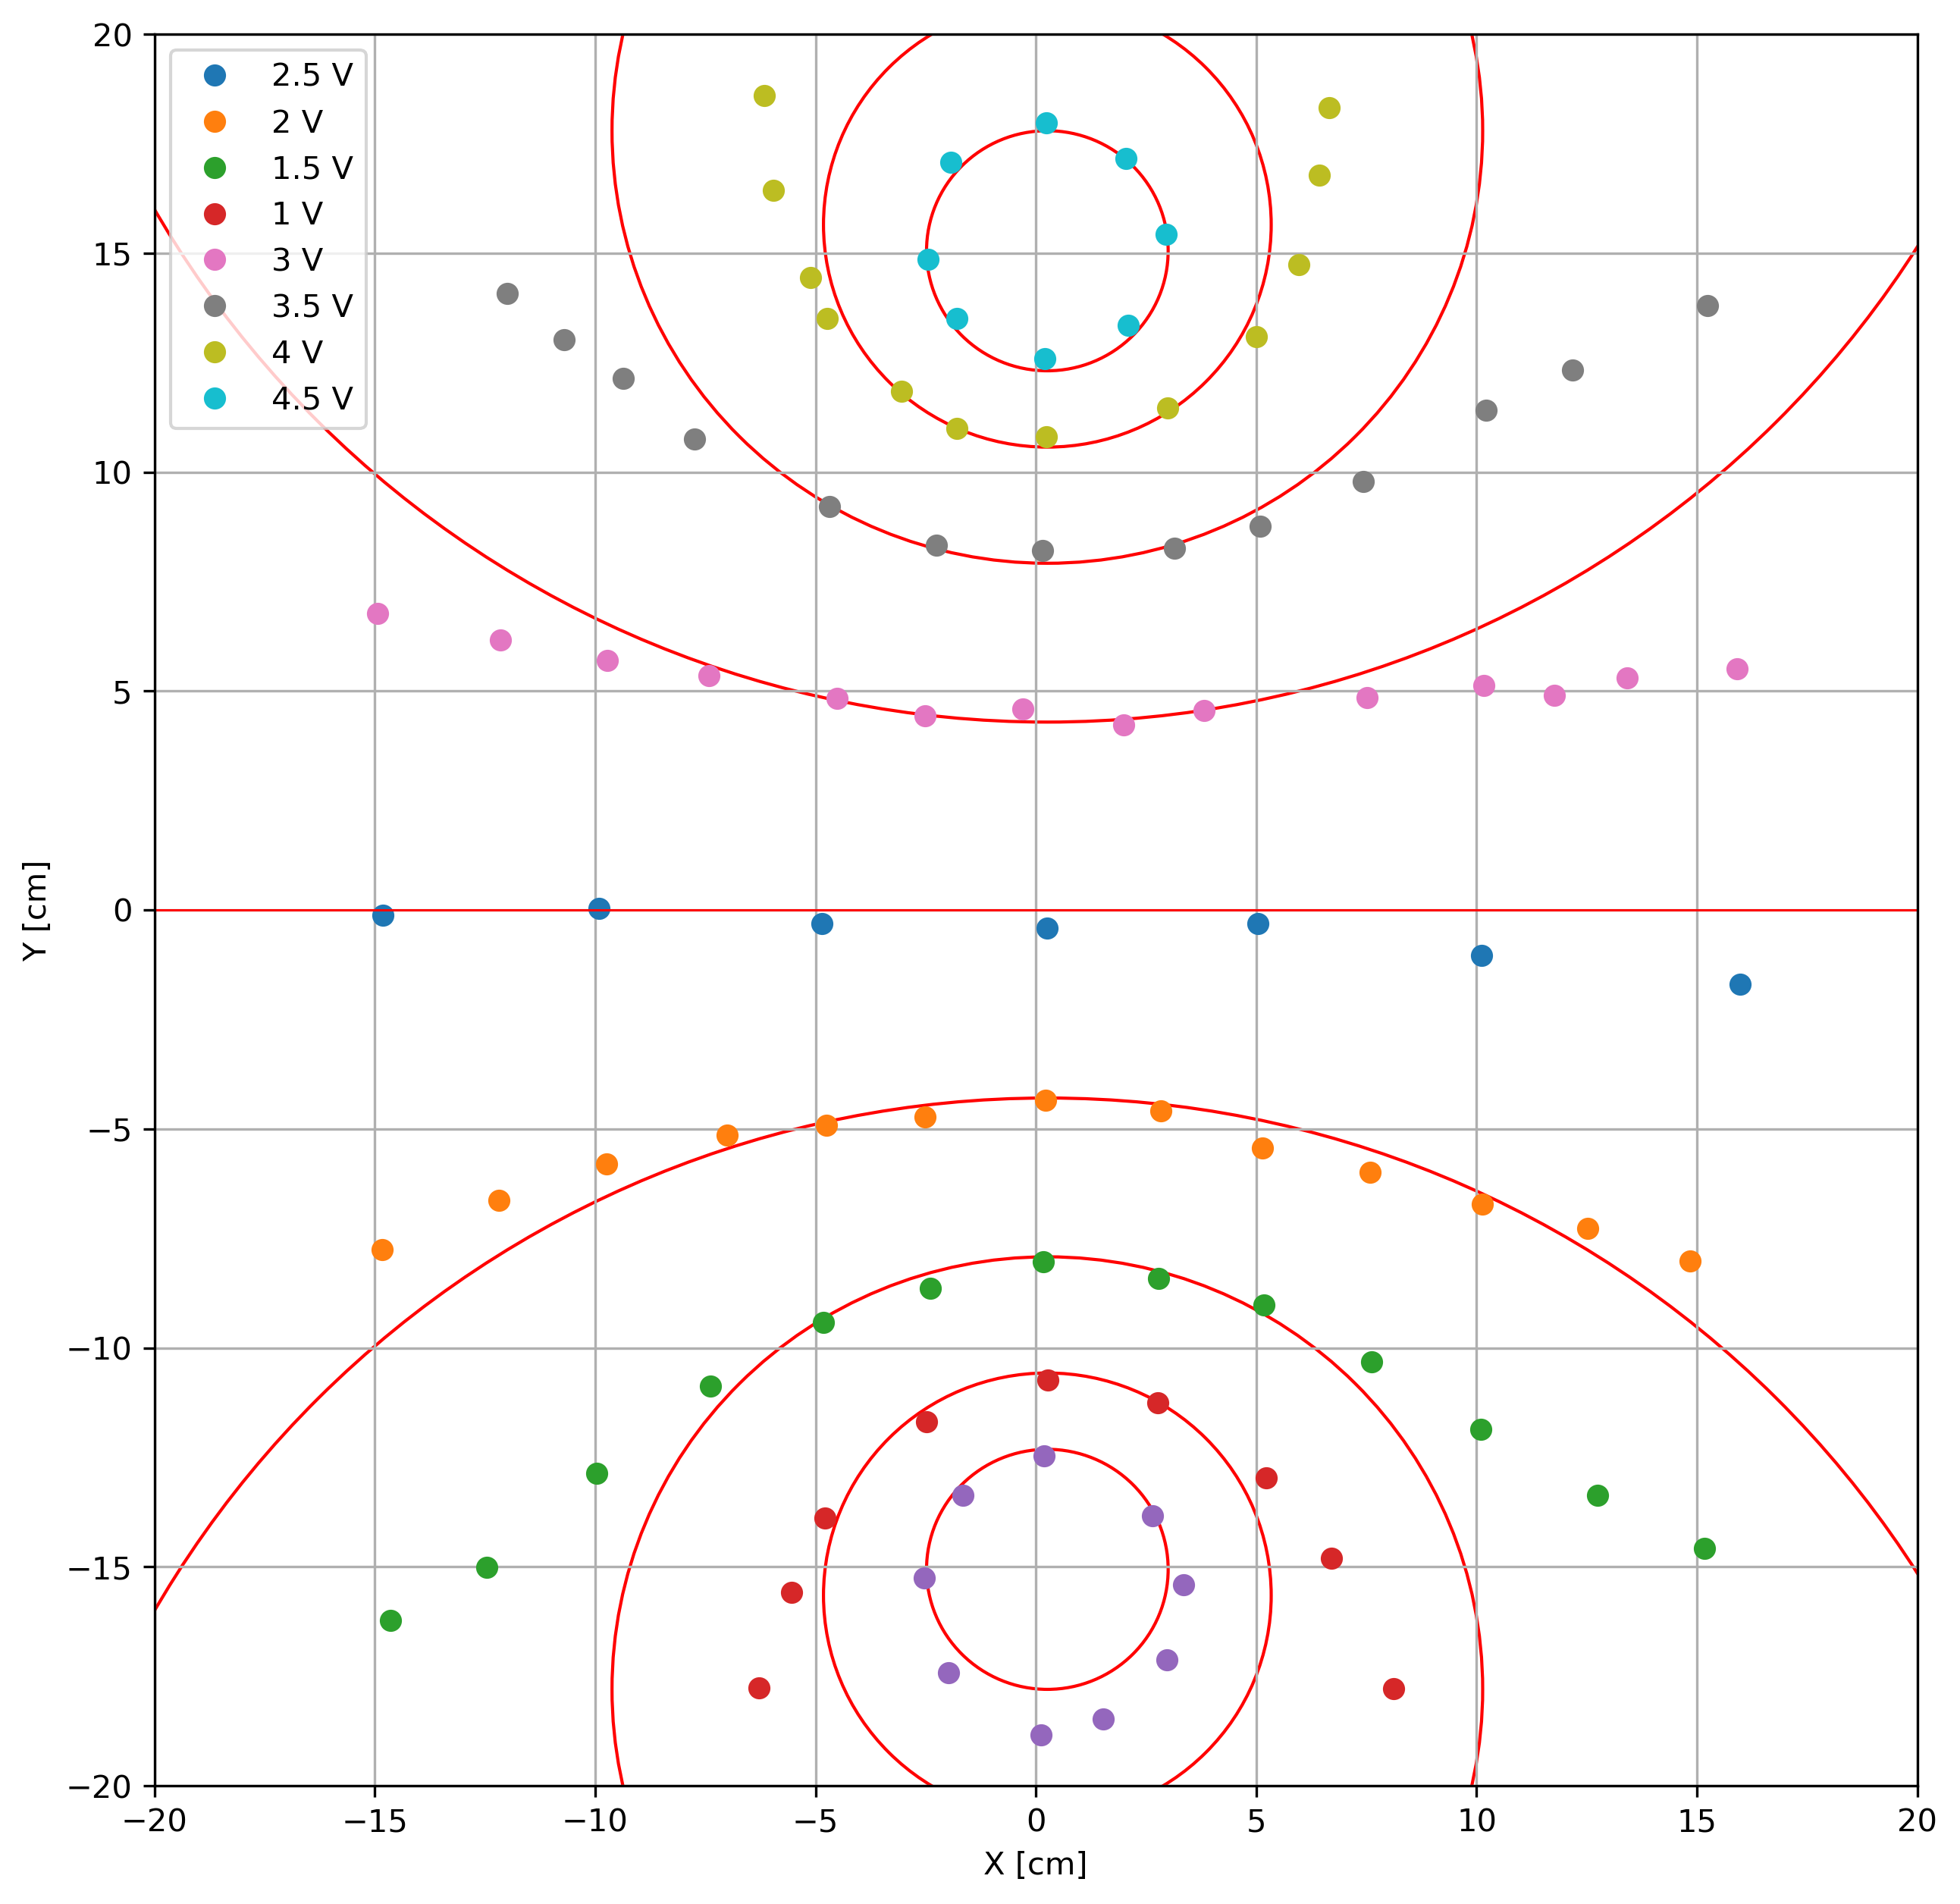
\includegraphics[max width=0.5\textwidth, center]{plot_high_res}
		\caption{Naměřené hodnoty ekvipotenciálních hladin a Apolloniovy kružnice těchto hladinám náležející}
		
	\end{center}
\end{figure}

	\section{Závěr}
	Z obr. 5 lze pozorovat, že naměřené hodnoty přesně nekopírují teorií předpokládané křivky. I přes intenzivní snahu kalibrovat měřicí systém (správně vyrovnat vanu a odstranit ruch z osciloskopu) nebylo možné hladiny určit jednoznačně. Ztrátu přesnosti s rostoucí vzdáleností od středu osy Y proto vyvozujeme i ze skutečnosti, že je rychlost změny pole dále od osy Y nižší, než na ní, a jelikož hledáme lokální extrém, jsou hodnoty v jeho blízkém okolí mnohem blíže sobě, než na ose Y. Pozorování takto malé změny již z velké části záleží i na přesnosti přístroje, která byla v tomto případě již za hranicí svých schopností. Tuto hypotézu by bylo zajímavé ověřit automatizací pokusu, kdy by se hodnoty rozdílů napětí automaticky ukládaly a elektrické pero se pohybovalo o jasne dané, malé vzdálenosti (samozřejmě za předpokladu, že se nám vanu podařilo bezchybně vyrovnat). Z toho by bylo možné vytvořit teplotní mapu pro určitý počet hladin a pozorovat, zda teorii odpovídá více. Jsme též přesvědčeni, že by přesnost měření mohla zvýšit vyšší amplituda napětí generovaného signálu, jelikož bychom nebyli již tolik limitováni přesností osciloskopu. 
		\end{multicols}
	
	\section{Použitý kód}
	{\tiny \begin{verbatim}
	
	import numpy as np
	import matplotlib.pyplot as plt
	import matplotlib.patches as patches
	
	import pandas as pd
	
	data = pd.read_csv("data.csv")
	
	U = 5
	h = 0.1488
	R = 0.015
	a = np.sqrt(h**2 - R**2)
	print ("a = ", a)
	# Create columns
	u = np.arange(0.5, 5, 0.5).reshape(-1, 1)
	ld = np.zeros((9,1)) 
	xs = np.zeros((9,1))  
	r = np.zeros((9,1))  
	
	# Concatenate the columns to form a new array
	new_array = np.hstack(( u, ld, xs, r))
	def update_cols(arr):
	arr[:, 1] = np.exp (( arr[:, 0] - U/2)/U * 2*np.log((h+a)/R))
	arr[:, 2] = a * (arr[:, 1]**2 +1)/(arr[:, 1]**2 -1) *100
	arr[:, 3] = np.sqrt((arr[:, 2]/100)**2 - a**2)*100
	return arr
	
	new_array = update_cols(new_array)
	print(new_array)
	df = pd.DataFrame(new_array, columns=[ 'U', 'lambda', 'xs[cm]', 'r[cm]'])
	
	############################################
	start = 2.45
	end = 2.551
	step = 0.001
	u = np.arange(start, end, step).reshape(-1, 1)
	zbytek = np.zeros((len(u),3)) 
	convarray = np.hstack(( u, zbytek))
	
	convarray = update_cols(convarray)
	convarray[50] = [0, 1, 0, 0]
	
	df2 = pd.DataFrame(convarray, columns=[ 'U', 'lambda', 'xs[cm]', 'r[cm]'])
	df2 = pd.concat([df2], ignore_index=True)
	print(df2)
	
	
	# Add a header row with labels
	df_with_header = pd.concat([ df], ignore_index=True)
	
	print(df_with_header)
	
	# the first column is 'label', the second column is 'x', and the third column is 'y'
	label_column = data.columns[0]
	x_column = data.columns[1]
	y_column = data.columns[2]
	center_y_column = df_with_header.columns[2]
	radius_column = df_with_header.columns[3]
	
	# Define a color map
	colors = plt.cm.get_cmap('tab10', 10)  # Get a colormap with 10 distinct colors
	
	# Plotting the data
	plt.figure(figsize=(10, 10))
	hladiny = ["2.5 V", "2 V", "1.5 V", "1 V","", "0.5 V", "3 V", "3.5 V", "4 V", "4.5 V"]
	
	# Group the data by the label column and plot each group with a different color
	for label, group in data.groupby(label_column):
		plt.plot(group[x_column], group[y_column], marker='o', linestyle='None', color=colors(label), label=hladiny[label])
	
	
	# Add circles to the plot using data from df_with_header
	ax = plt.gca()  # Get the current axes
	for _, row in df_with_header.iterrows():
		circle = patches.Circle((0.26, row[center_y_column]), row[radius_column], edgecolor='r', facecolor='none')
		ax.add_patch(circle)
	
	plt.axhline(y=0, color='r', linestyle='-', linewidth=0.6)
	
	
	# Customize the plot
	plt.xlim(-20, 20)
	plt.ylim(-20, 20)
	plt.xlabel('X [cm]')  
	plt.ylabel('Y [cm]')  
	plt.legend()
	plt.grid(True)
	
	plt.savefig('plot_high_res.png', format='png', dpi=300, bbox_inches='tight')
	# Show the plot
	plt.show()
	
	############################################
	
	
	
	center_y_column = df2.columns[2]
	radius_column = df2.columns[3]
	
	
	
	
	# Create multiple graphs, each plotting just two circles
	num_rows = len(df2)
	
	for i in range(num_rows//2):
		plt.figure(figsize=(10, 10))
	
	# Add two circles to the plot using data from df_with_header
	ax = plt.gca()  # Get the current axes
	indices = [i, num_rows-1 - i]
	for idx in indices:
		row = df2.iloc[idx]  # Use iloc to access rows by integer-location based index
		circle = patches.Circle((0, row[center_y_column]), row[radius_column], edgecolor='r', facecolor='none')
		ax.add_patch(circle)
	
		# Customize the plot
		plt.xlim(-20, 20)
		plt.ylim(-20, 20)
		plt.xlabel('X [cm]')  # Corrected column name
		plt.ylabel('Y [cm]')  
		plt.legend([f'U = ± {df2.iloc[indices[0], 0]:.3f}V'])
		plt.grid(True)
	
		# Save the plot as a high-resolution image
		plt.savefig(f'plot_{i}.png', format='png', dpi=300, bbox_inches='tight')
	
		# Show the plot (optional, can be commented out if not needed)
		#plt.show()
	
		# Close the plot to free up memory
		plt.close()
	
	\end{verbatim}}

	
	

	
	% Nakonec nezapomeňte projet text programem vlna nebo vlnka, např.
	% 	vlna -m -l -n mojeuloha.tex
	% nebo zkontrolovat a opravit jednopísmenné předložky na koncích řádků ručně.
	
\end{document}
